\section{Results/Analysis}

\subsection{Comparison between frameworks}
To compare between CNN frameworks, AlexNet was trained for many iterations on each framework.
The whole process was profiled, and one mini-batch iteration was selected for analysis after the time metrics were stabilized.
Model parameters and hyperparameters of the solver are carefully equalized previously in order to remove the effect from things other than the framework itself.
The result is shown in Figure~\ref{fig_time_frameworks}.

\begin{figure*}
  \centering
  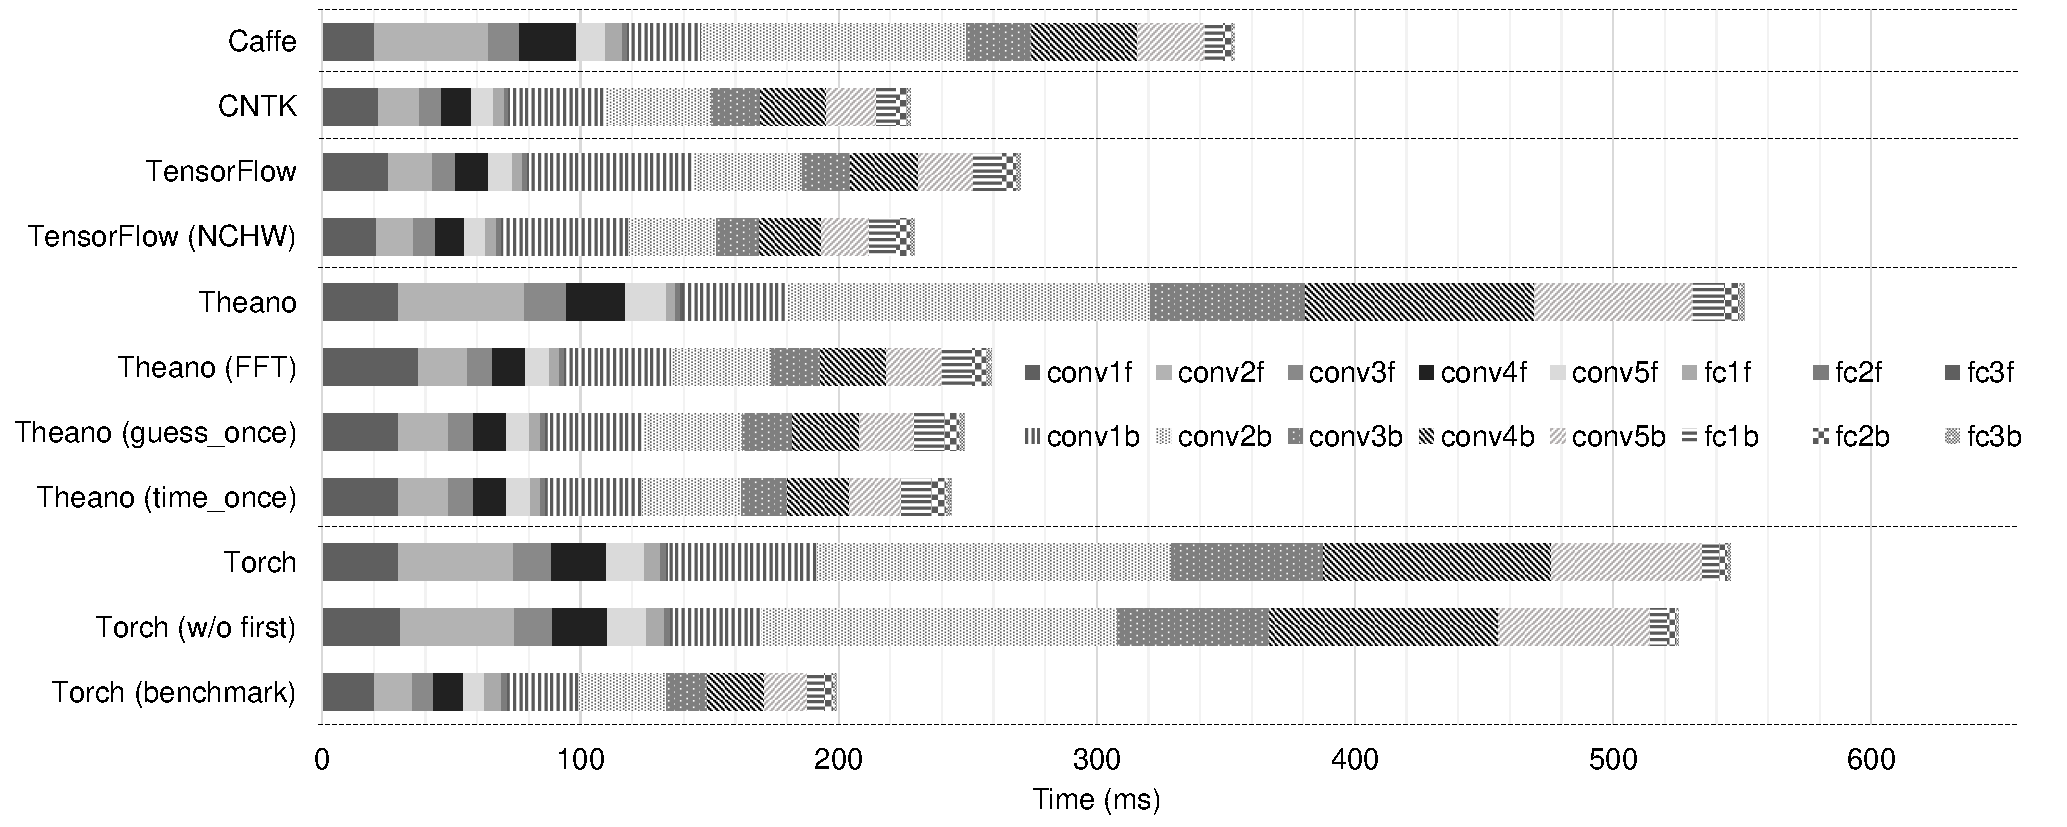
\includegraphics[width=\linewidth]{./figures/time_frameworks}
  \caption{%
Layer-wise time of AlexNet training under various framework configurations.
In the legend, `conv' means convolution layer and `fc' means fully-connected layer.
Numbers mean the layer order in AlexNet.
Suffix `f' means forward propagation, and `b' means backward propagation.
Each alphabet means the following: A = Caffe, B = TensorFlow (default), C = TensorFlow (with NCHW tensor format), D = Theano (default), E = Theano (FFT), F = Theano (guess\_once), G = Theano (time\_once), H = Torch (default), I = Torch (no backward data convolution in the first layer), J = Torch (FFT), K = Torch (benchmark option).
\label{fig_time_frameworks}
  }
\end{figure*}

First, we focused at how each framework chose kernels.
Caffe did not provide any user options to affect kernel choices.
Instead, Caffe depended on cuDNN's heuristics, which try to determine the best suited algorithm under the given specification.
Surprisingly, Caffe did not have appropriate memory strategy for kernels yet, just passing 8MB workspace limit as an argument.
Low-memory required algorithms, such as GEMM and Winograd, were selected, resulting in low performance compared to other frameworks.
Tensorflow also did not provide options for kernel choices.
Unlike Caffe, however, it executed all available algorithms on the first run by itself.
Only the fastest kernels in each layer were executed for subsequent runs.
Under the AlexNet, FFT algorithms were chosen for all convolution layers except the first layer, where FFT cannot be used due to stride of 4.
One downside was that algorithms were chosen from hardcoded set, so recently added option (like WINOGRAD\_NONFUSED) was not included.

On the other hand, Theano provide full access on the kernel choices.
We could specify convolution algorithms to be used, globally or layer-by-layer.
We found layerwise option is better, since implicit GEMM is chosen as fallback if the layer specification does not match global option, and it can even be slower than explicit GEMM which is the default option.
This is the reason why the first layer of E in Fig~\ref{fig_time_frameworks} is slower than F, G, and even D.
Theano also had `guess\_once' option, which depended on cuDNN's heuristics like Caffe but provided proper arguments.
`time\_once' option was provided, too, which depended on cuDNN's functionality that run all available convolution algorithms and chose the fastest one.
Theano did not have downside like TensorFlow had, because it directly used cuDNN's API\@.
If `time\_once' option was on, it used GEMM on the first layer and had mixed use of FFT and Winograd on the rest convolution layer.
When `guess\_once' option was on, it used slightly different kernels but showed almost identical running time with `time\_once' option, proving that heuristic of cuDNN is quite reliable.
Although Theano executed the fastest convolution kernels, Theano did not have the fastest convolution when it came to the whole layer.
Theano used its own runtime-compiled kernels for bias addition and ReLU activation, and they were more than twice slower than cuDNN's or other libraries'. (Table~\ref{table_misc_kernel})
Torch provided full control on the kernel choices, similar to Theano.
Torch's cuDNN backend, cudnn.torch, had cudnn.benchmark option which is the same with `time\_once' in Theano.
When benchmark option is on, Torch showed overall fastest execution time among four frameworks.

\begin{table*}[]
\centering
\caption{Misc.\ kernels}
\label{table_misc_kernel}
\begin{tabular}{llllll}
\multicolumn{2}{l}{Framework} & Caffe & TensorFlow & Theano & Torch \\ \hline
Bias addition    & From       & cuDNN & TensorFlow & Theano & cuDNN \\
                 & Time (ms)  & 2.64  & 2.84       & 7.88   & 2.63  \\
ReLU activation  & From       & cuDNN & Eigen      & Theano & cuDNN \\
                 & Time (ms)  & 2.56  & 2.43       & 4.59   & 2.56 
\end{tabular}

This table is about kernels included in convolution layers, but not directly participating in convolutions.
`From' means which library kernels came from.
Times are measured in the first convolution layer.
Noticeably, Theano uses kernels which are compiled in runtime and they are quite slow compare to others.
\end{table*}

We also found a few phenomenons in terms of framework overhead.
The most noticable one was the tensor format.
Caffe, Theano, and Torch used NCHW tensor format, which means (batch, channel, height, width) dimensions.
Tensorflow supported NCHW, but it used NHWC more popularly.
Its tutorial codes used NHWC format, and many functions, like conv2d, used NHWC as a default argument.
While NHWC can be faster when there are channel-wise operations, some cuDNN's convolution kernels (such as FFT) only support NCHW format.
Besides, TensorFlow always do NHWC-to-NCHW dimension swap even if it is using NHWC-supported kernels.
Therefore, using NHWC tensor format leads to intensive dimension swapping before and after the convolution.
In our AlexNet, just changing tensor format from NHWC to NCHW led to about 15\% improve in speed on TensorFlow.

Second issue was backward data convolution in the first convolution layer.
The first layer does not have previous layer to update parameters, so it does not need backward data convolution, which basically calculates output gradients for the previous layer.
Caffe and Theano automatically did not execute the operation, and it can be disabled by setting gradInput of the first layer to nil.
On TensorFlow, however, backward data and filter convolution of the first layer are always done together to prevent non-reproducibility due to race condition. (See gate\_gradients parameter in tf.train.Optimizer.compute\_gradients.)
This made TensorFlow slower than Torch, which is almost identical in terms of kernel choices.
It can be disabled at the expense of reproducibility and accurate gradients, although we left it enabled.

%그 외 사소한 것으로 텐서에 네트워크 입력을 feed_dict로 주면 CPU 복사가 일어나서 매우 느리므로 FixedLengthRecordReader 등으로 주는게 좋다.
%https://github.com/tensorflow/tensorflow/issues/2919

%https://github.com/BVLC/caffe/blob/rc3/src/caffe/layers/cudnn_conv_layer.cpp#L113
%https://github.com/tensorflow/tensorflow/blob/v0.10.0rc0/tensorflow/core/kernels/conv_ops.cc#L460
%https://github.com/tensorflow/tensorflow/blob/v0.10.0rc0/tensorflow/stream_executor/cuda/cuda_dnn.cc#L933
%https://github.com/Theano/Theano/blob/rel-0.8.2/theano/sandbox/cuda/dnn.py#L285
%https://github.com/Theano/Theano/blob/rel-0.8.2/theano/sandbox/cuda/dnn_fwd.c#L227
%https://github.com/soumith/cudnn.torch/blob/R5/SpatialConvolution.lua#L166

\subsection{Characterization of different convolution algorithms}
Since forward and backward propagation of convolution layers takes most of the running time, we run the same model on different convolution kernel to characterize the performance of each convolution algorithm.
Three types of convolutions are computed for each iteration.
Forward convolution (FWD) computes the layer output, backward data convolution (BD) computes backward gradient input and backward filter convolution (BW) computes gradients of network parameters.
CuDNN R5 supports matrix multiplication convolution (GEMM), FFT convolution, and Winograd convolution.
CuDNN has various GEMM convolution algorithms and the tested algorithm is implicit GEMM precomp algorithm.
The Winograd kernel used in the analysis is Winograd nonfused kernel which was recently implemented  on cuDNN 5.1.
Since the first convolution layer has stride of 4, Winograd and FFT convolution cannot be applied.
Therefore GEMM convolution algorithm is applied on the first convolution layers of Wingrad and FFT convolution experiment.
Direct convolution is tested by Torch binding of Cuda-convnet3.
All comparisons are done on Torch 7 because currently it is the only framework which officialy supports newest versions of cuDNN and Cuda-convnet3.
Randomly generated batch inputs are used to remove IO latency.

\begin{figure*}[!t]
  \centering
  \subfloat[Forward execution time] {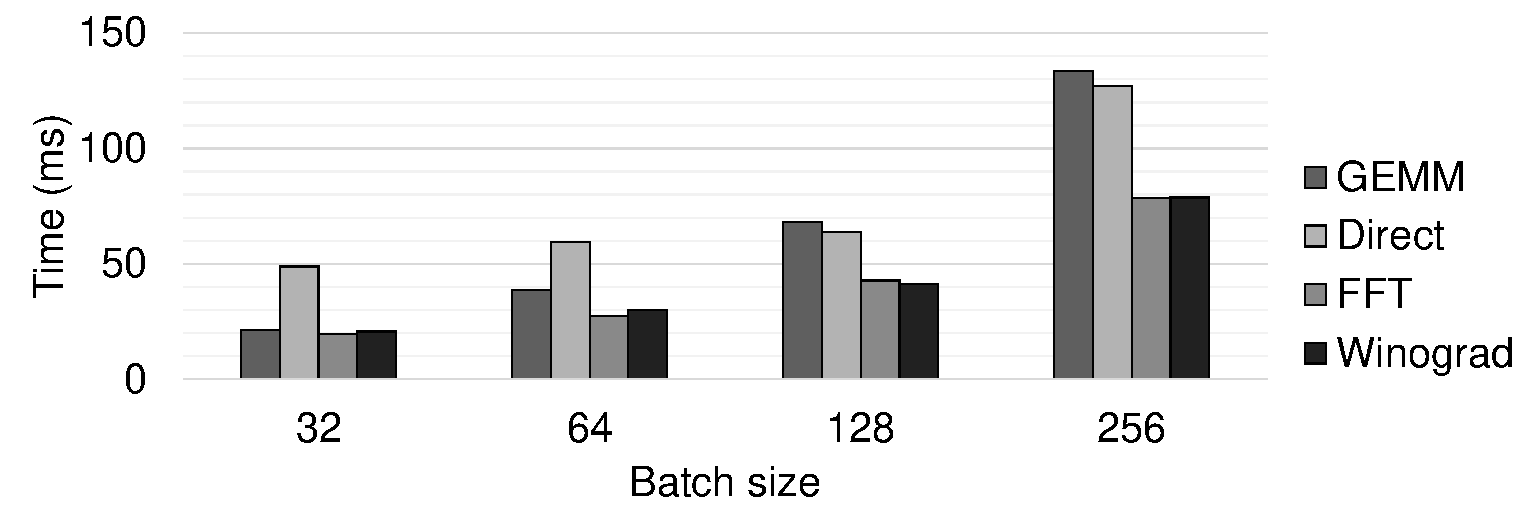
\includegraphics[width=.45\linewidth]{./figures/gpu_time_fwd}
  \label{fig_gpu_time_fwd}}
  \subfloat[Backpropagation execution time] {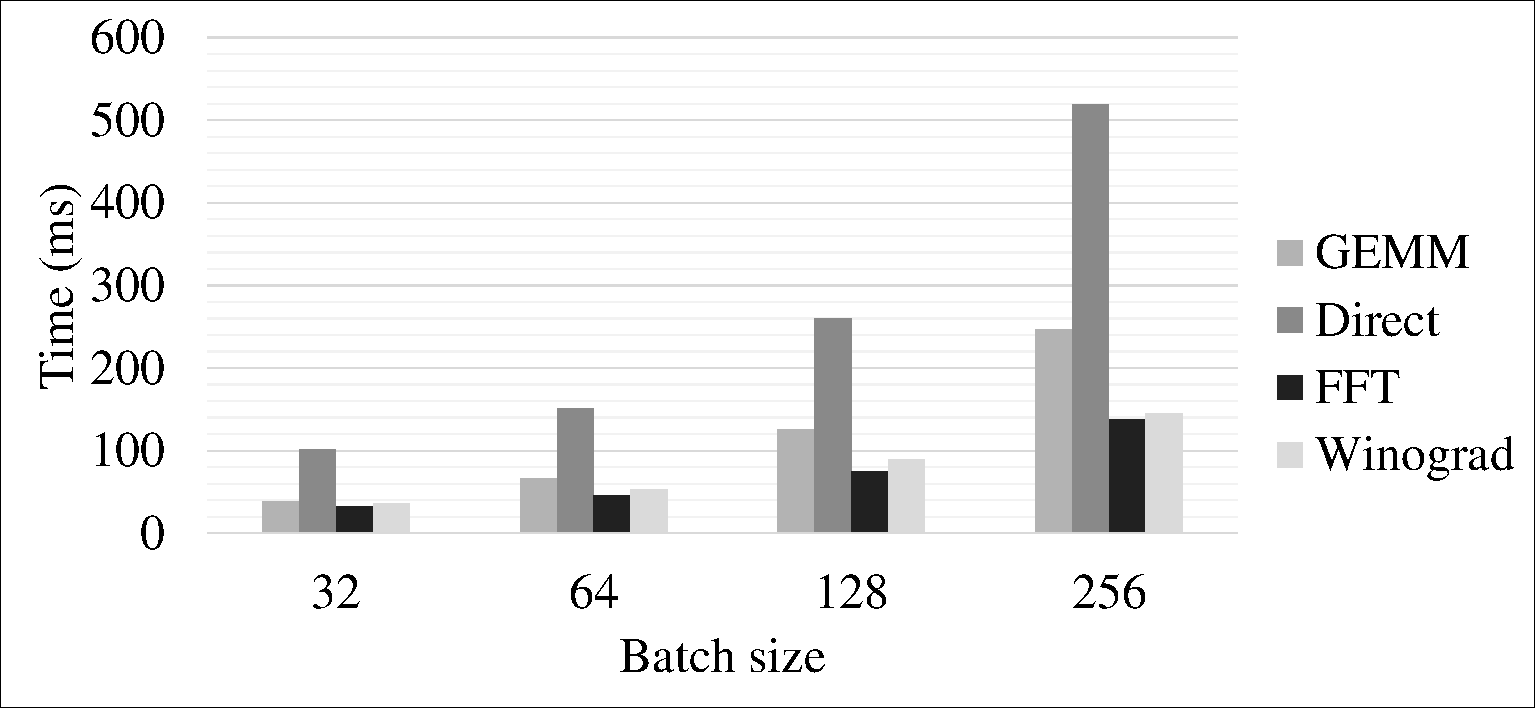
\includegraphics[width=.45\linewidth]{./figures/gpu_time_bwd}
  \label{fig_gpu_time_bwd}}
  \hfil
  \subfloat[Forward execution time from conv3 to conv5 layer] {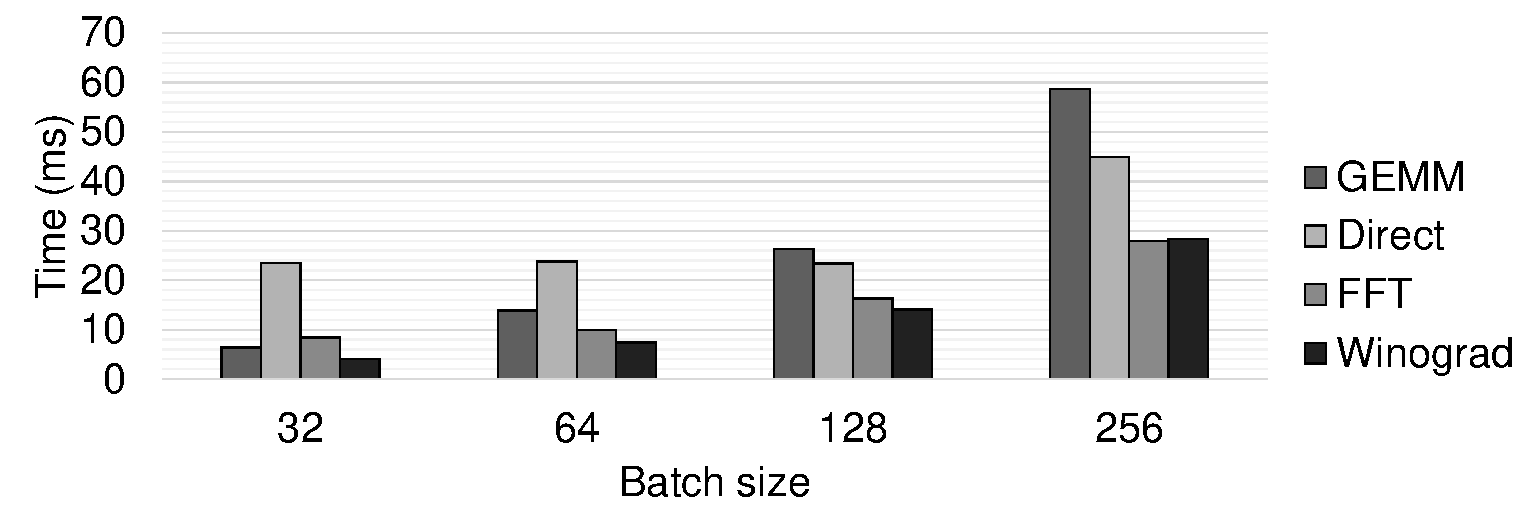
\includegraphics[width=.45\linewidth]{./figures/gpu_time_conv345}
  \label{fig_gpu_time_conv345}}
  \subfloat[Memory usage] {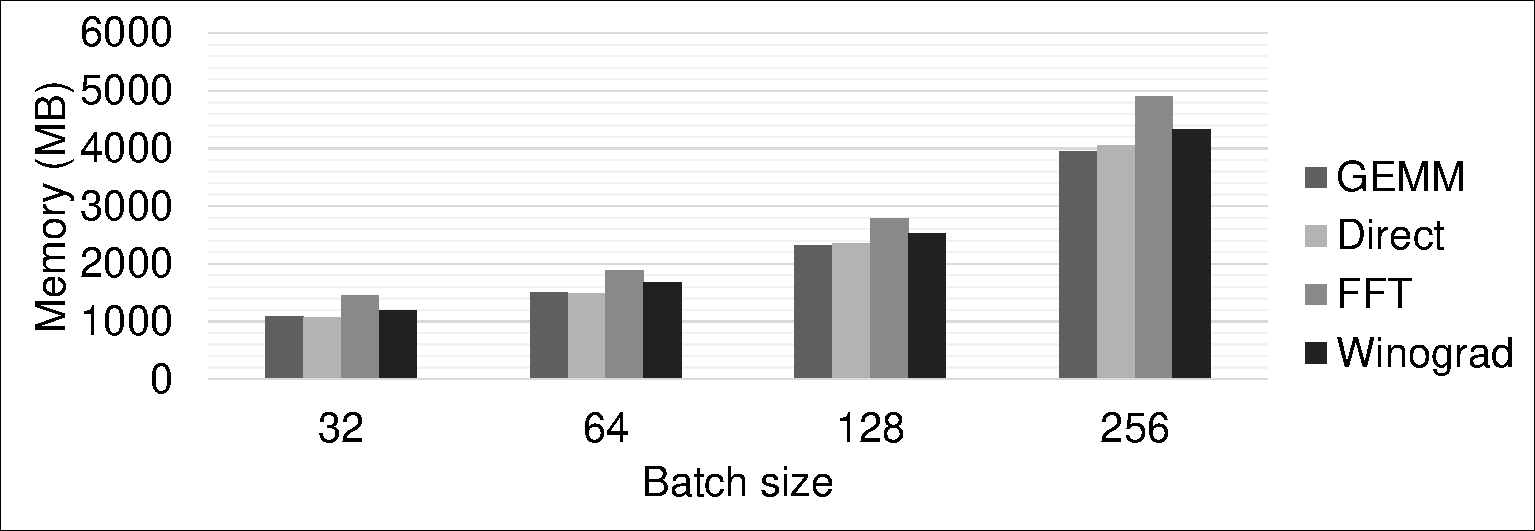
\includegraphics[width=.45\linewidth]{./figures/gpu_mem_kernels}
  \label{fig_gpu_mem}}
  \caption{Execution time and memory usage comparison of convolution kernels.}
  \label{fig_conv_time}
\end{figure*}

Fig~\ref{fig_conv_time} shows execution time comparisons between convolution kernels.
The forward and backward propagation time is measured as average of 100 iterations.
Winograd convolution and FFT convolution perform better than direct or GEMM convolution most of the time.
Since many recent CNN models use 3x3 filter for convolution layers\cite{vgg}, the forward propagation times of convolution layer 3 to 5 are separately tested and the result is on Fig~\ref{fig_gpu_time_conv345}.
With respect to total training time, FFT is the fastest among all batch sizes.
But for 3x3 convolution layers, Winograd convolution performs better on smaller batch sizes.
Winograd convolution performs better on small batch sizes, while FFT scales better on bigger batch sizes.
Cuda-convnet scales bad when the batch size is smaller than 128 while GEMM convolutoin sclaes almost linearly.
Theoretically forward and backward propagation are symmetric.
Since backpropagation executes 2 convolutions per layer, the backpropagation time should be a double of forward propagation time.
While most other algorithms follow this rule, direct convolution kernels do not.
Backpropagation execution time of direct convolution is around a quadruple of forward propagation time.
Fig~\ref{fig_gpu_mem} shows peak GPU device memory usage for each convolution algorithms.
FFT convolution kernels occupies the most GPU memory, using around 20\% more memory than GEMM convolution kernels.

\begin{figure*}[!t]
  \centering
  \subfloat[Forward execution time] {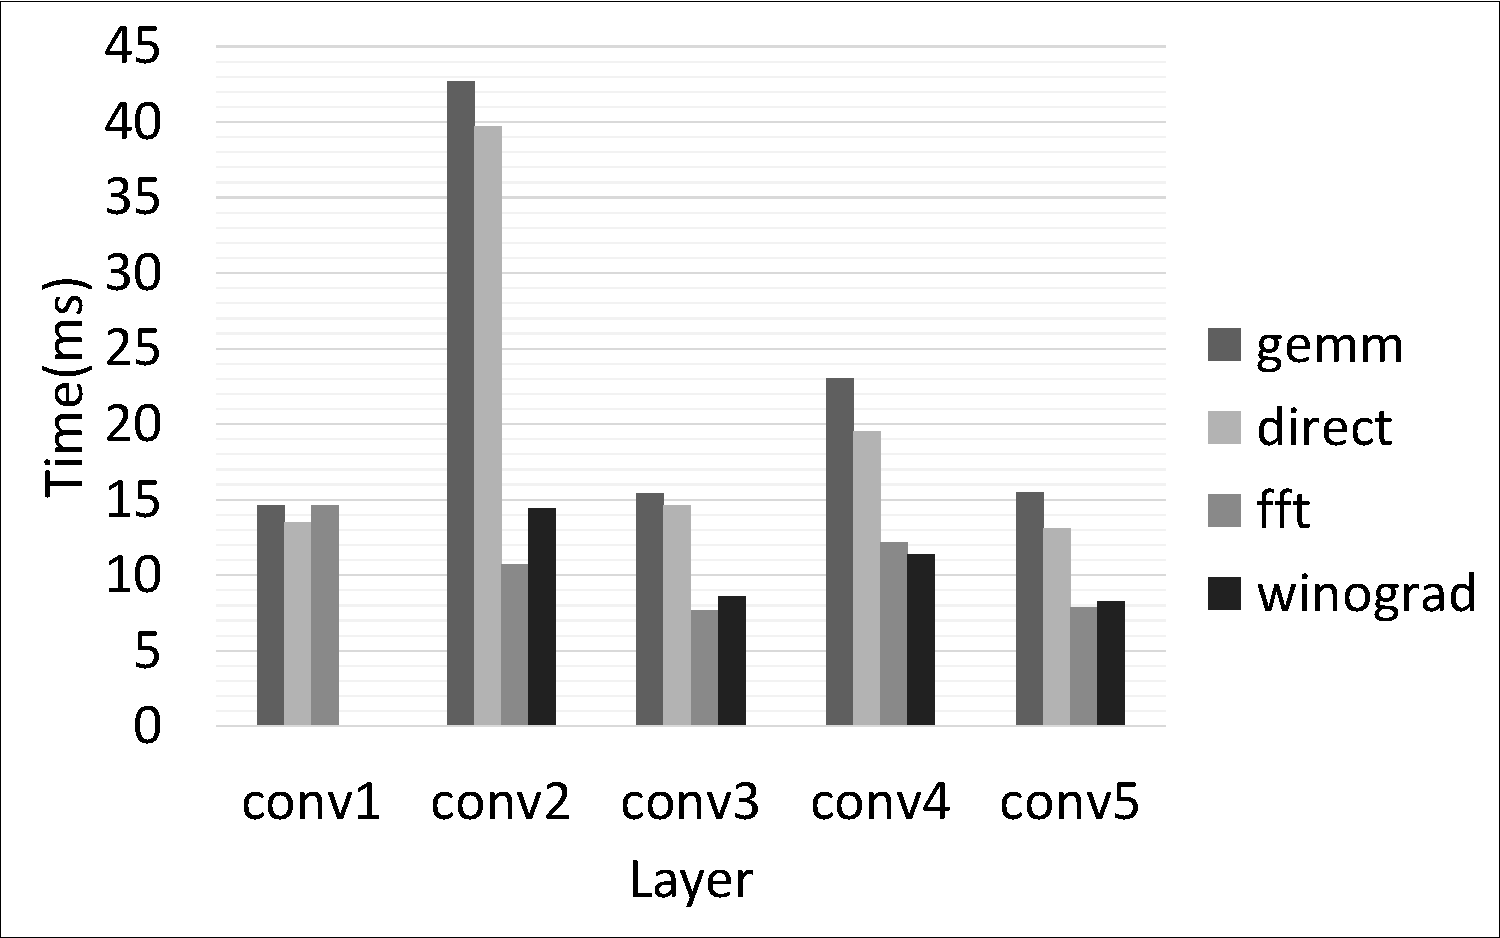
\includegraphics[width=.32\linewidth]{./figures/layerwise_fwd}
  \label{fig_layerwise_fwd}}
  \subfloat[Backward Data execution time] {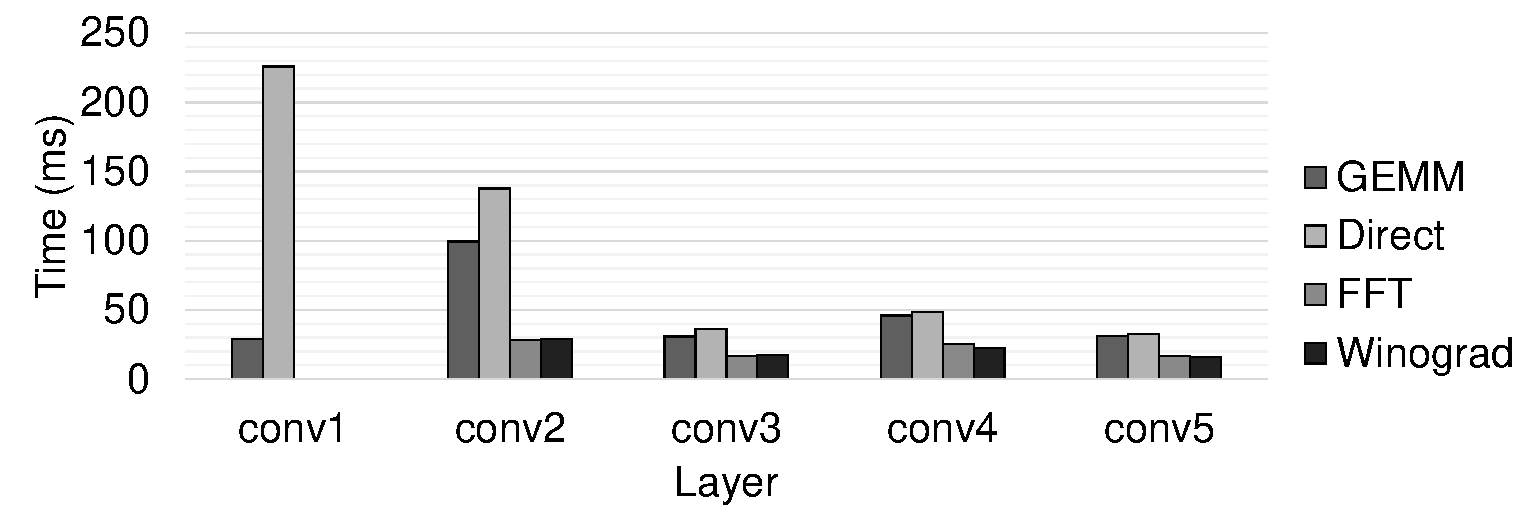
\includegraphics[width=.32\linewidth]{./figures/layerwise_bd}
  \label{fig_layerwise_bd}}
  \subfloat[Backward Filter execution time] {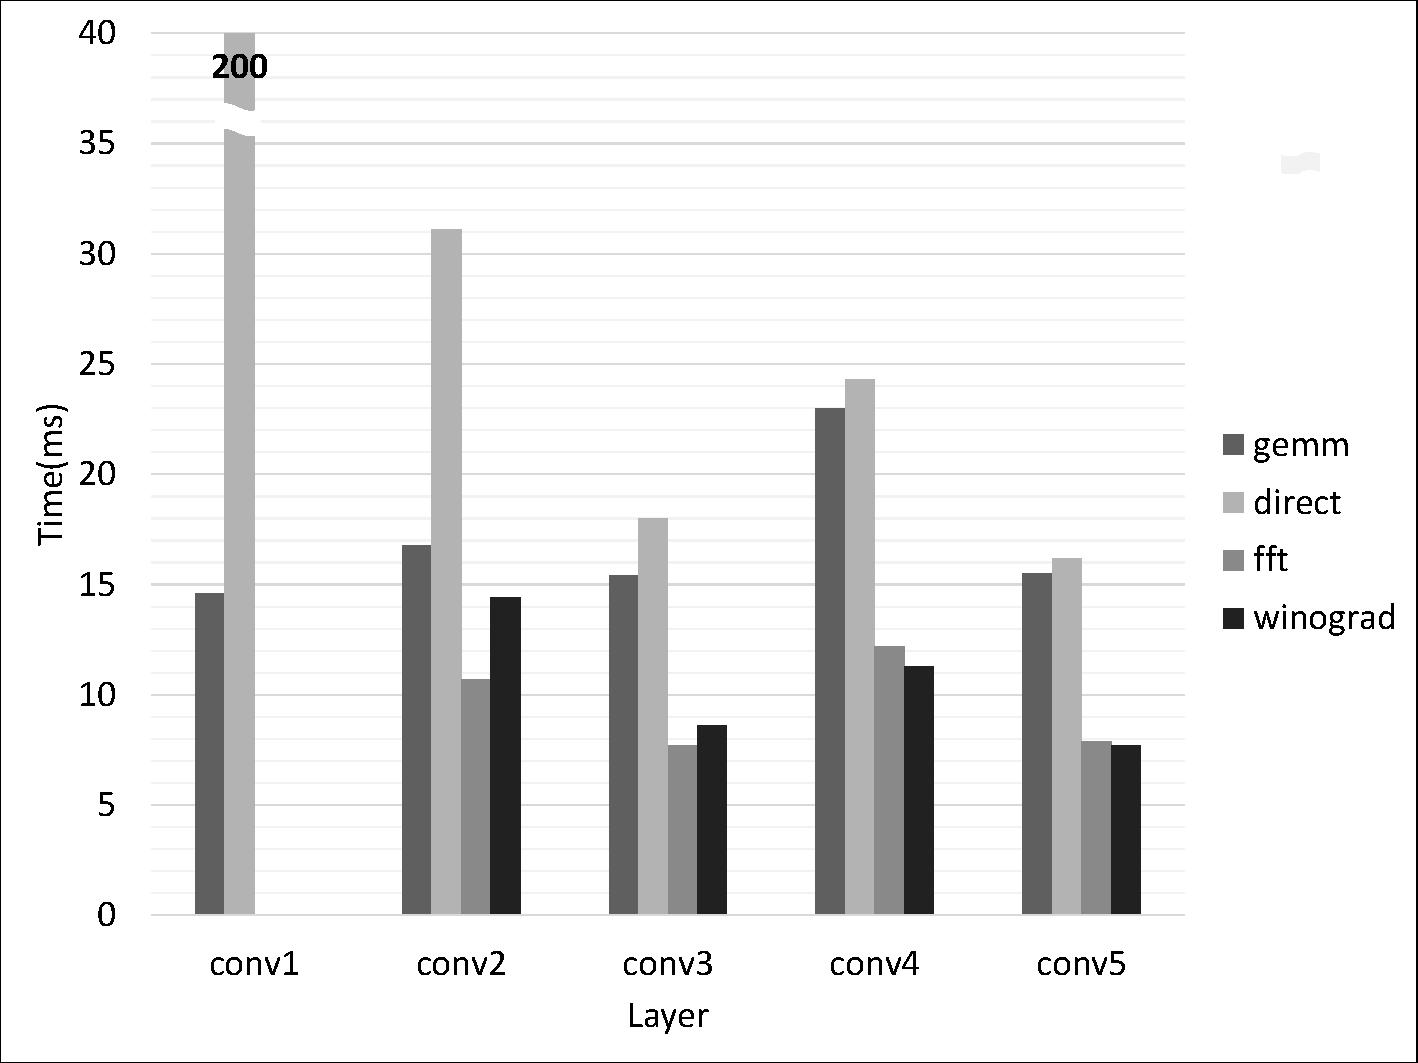
\includegraphics[width=.32\linewidth]{./figures/layerwise_bw}
  \label{fig_layerwise_bw}}
  \hfil
  \subfloat[Forward floating point operations count] {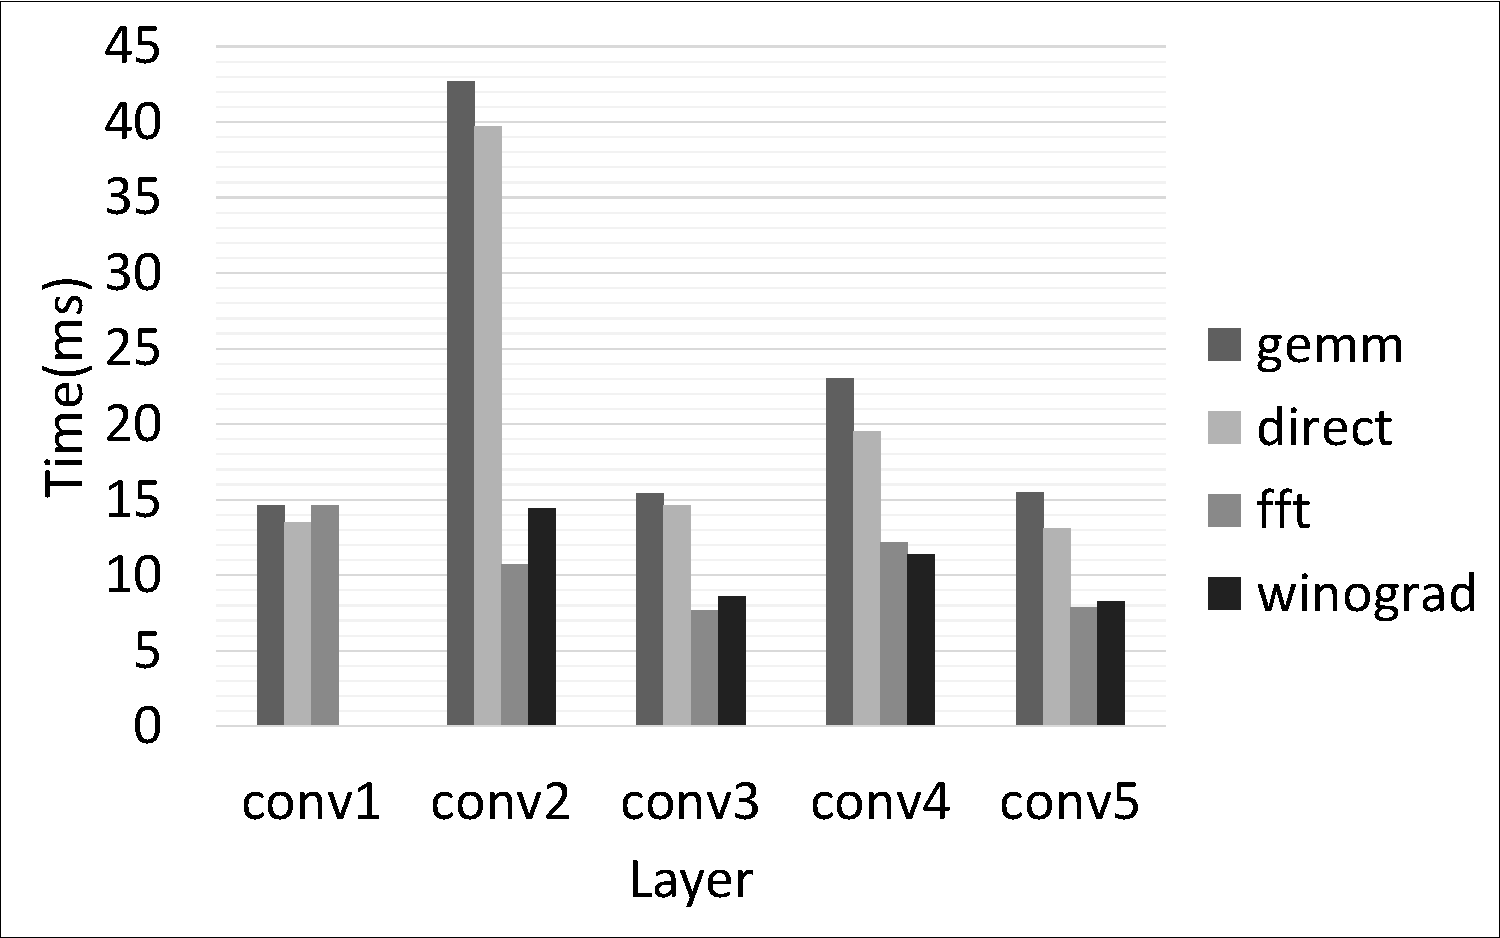
\includegraphics[width=.32\linewidth]{./figures/layerwise_fwd}
  \label{fig_layerwise_flop_count}}
  \subfloat[Forward Flops throughput] {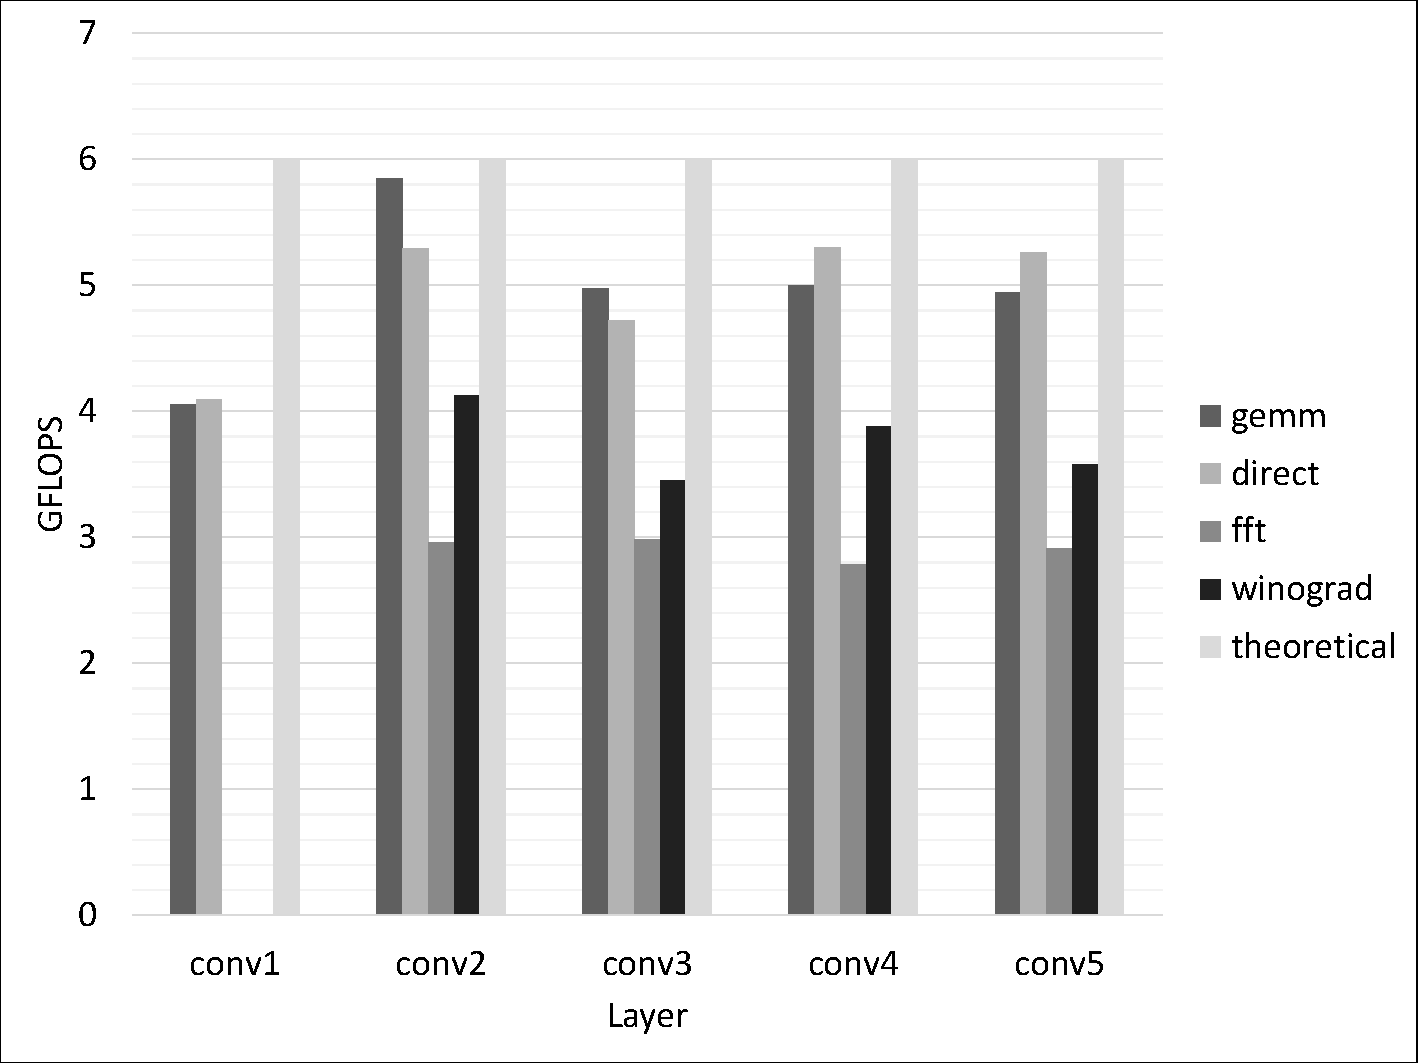
\includegraphics[width=.32\linewidth]{./figures/layerwise_flops_fwd}
  \label{fig_layerwise_flops_fwd}}
  \subfloat[Backward Flops throughput] {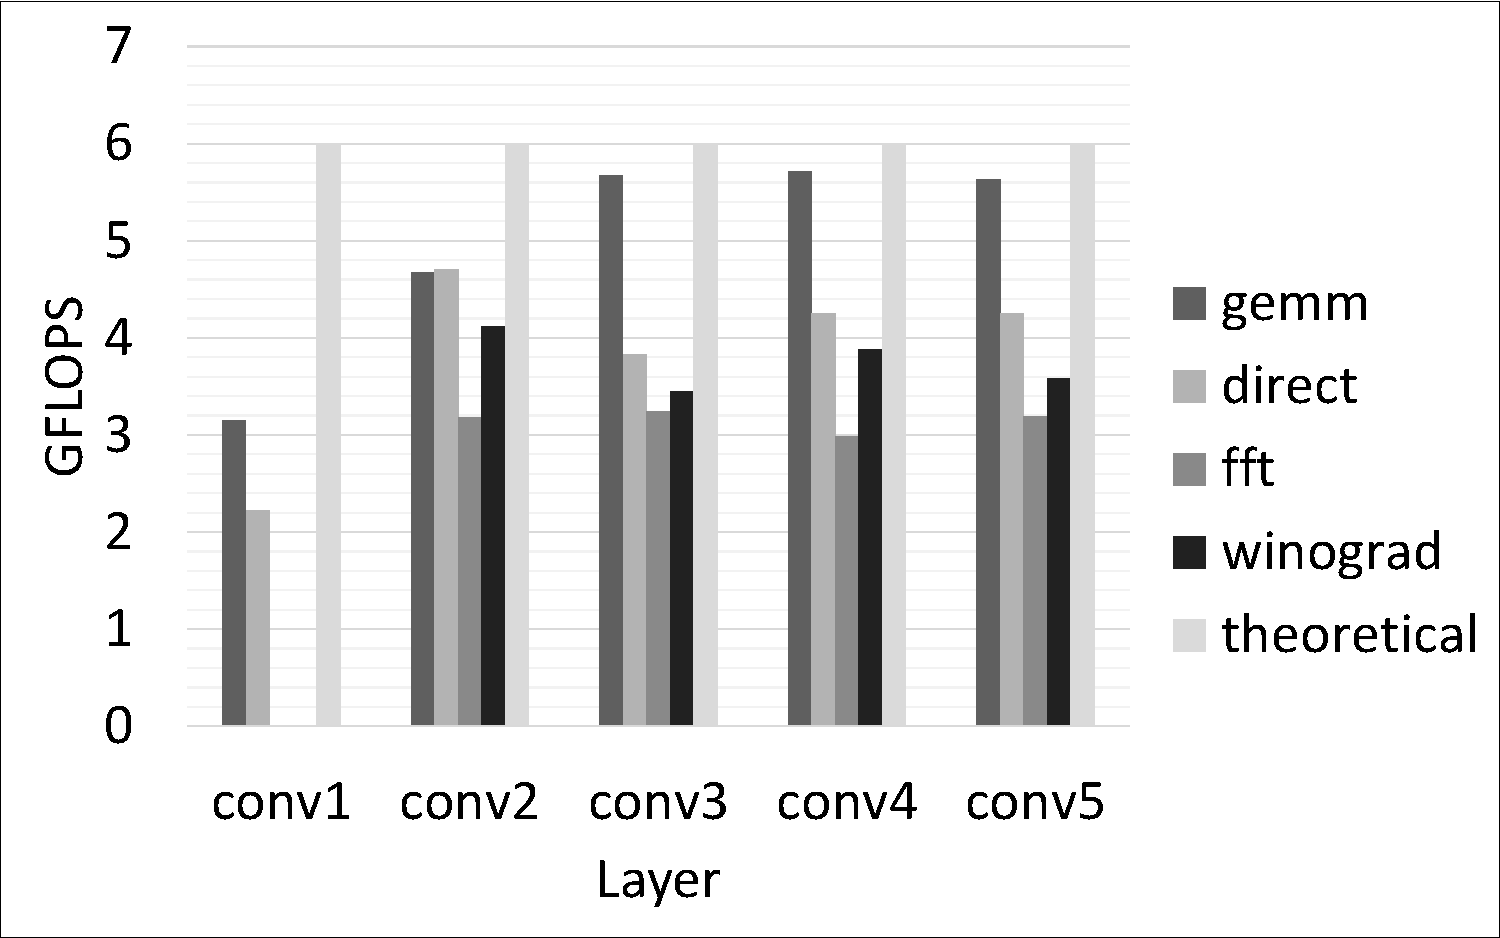
\includegraphics[width=.32\linewidth]{./figures/layerwise_flops_bd}
  \label{fig_layerwise_flops_bd}}
  \caption{Layerwise analysis of convolution kernels}
  \label{fig_layerwise}
\end{figure*}

Fig~\ref{fig_layerwise} shows layerwise analysis of convolution algorithms.
The batch size for layerwise comparison is set to 256.
The compute times and statistics of kernels are measured by NVIDIA nvprof profiler.
The main performance limiter for backpropation of Cuda-convnet is backward filter convolution on conv1 layer.
We expect that reason for the slow execution is low parallelism of kernels.
The backward direct convolution kernels have small thread numbers compared to other algorithms, generating 6 times smaller thread grid size.
The backward filter convolution for the first layer generates only 1024 threads, while Titan X has 3072 CUDA cores.

Fig~\ref{fig_layerwise_flop_count} compares floating operation counts of the convolution kernels measured by Nvidia's Cuda profiler.
The theoretical floating point operation counts are calculated as 2 * K*CRR*NWW since each calculation uses 1 addition and 1 multiplication.
FFT convolution consists of 1 filter flip kernel, 2 FFTs and 1 complex GEMM kernel.
Similarily nonfused Winograd convolution consists of 3 Tiling kernels and 36(in case of 3x3 filter) or 167(in case of 5x5 filter) GEMM kernels.
The statistics of those kernels are added up together per layer for the result.
Flops throughputs of the kernels shown in Fig~\ref{fig_layerwise_flops_fwd} and Fig~\ref{fig_layerwise_flops_bd} are calculated as Flop count/execution time.
Compared to maximum Flops throughput of Nvidia TitanX is 6TFlops, most convolution kernels show throughput more than 3TFlops.
The Flops throughput result indicate that convolution kernels are compute bounded rather than memory.
Even if FFT has slower Flops throughput, FFT convolution is usually the fastest due to much less algorithm complexity.
Especially on convolution layer 2 which uses 5x5 filter for convolution, FFT convolution is much faster than other algorithms becuase computation complexity of FFT does not depend on filter sizes.
Winograd's filtering algorithm also reduces Flop count by more than half makes perform similar to FFT convolution on convolution layers with 3x3 filters.

\subsection{Multi-GPU analysis}

To analyze multi-GPU scalability of frameworks, AlexNet was trained on each framework with 1 GPU, 2 GPUs, and 4 GPUs\@.
We adopted data-parallelism approach, which means that the same model resides in each GPU and input data is divided equally to feed GPUs.
After forward-backward propagation in each GPU, gradients should be accumulated in one GPU for gradient update.
If gradients are gathered sequentially (i.e., $GPU_1$ to $GPU_0$, then $GPU_2$ to $GPU_0$, \ldots), it takes $(N-1)$ gradients transfer time.
However, if gradients are accumulated in a fashion noted at Figure~\ref{fig_multigpu_algorithm}, it takes $\log{N}$ gradients transfer time, under the assumption that transfers can be parallelized if source and destination GPUs are distinct.
The assumption depends on hardware configuration, so we configured hardwares to support parallel transfers.
Regarding frameworks, Caffe natively supports the multi-GPU algorithm mentioned above.
In Torch and TensorFlow, we implemented the algorithm ourselves.
Theano did not support multi-GPU, so was not tested.
For training in each GPU, we selected the fastest option based on the our framework comparison experiments.

\begin{figure}
\begin{algorithmic}[1]
  \REQUIRE N = the number of GPU
  \REQUIRE B = batch size
  \STATE Run forward and backward propagation on each GPU with batch size of $B/N$.
  \STATE $p\gets 1$
  \WHILE[Sum reduction in $O(log N)$]{$p\not=2^{N}$}
    \STATE $i\gets 0$
    \WHILE[can be parallelized]{$i\not=N$}
      \STATE Add $GPU_{i+p}$'s gradients to $GPU_{i}$
      \STATE $i\gets i+p*2$
    \ENDWHILE
    \STATE $p\gets p*2$
  \ENDWHILE
  \STATE Do SGD on $GPU_{0}$.
  \STATE $p\gets 2^{N}$
  \WHILE[Propagate updated gradients.]{$p\not=1$}
    \STATE $p\gets p/2$
    \STATE $i\gets 0$
    \WHILE[can be parallelized]{$i\not=N$}
      \STATE Clone $GPU_{i}$'s gradients to $GPU_{i+p}$
      \STATE $i\gets i+p*2$
    \ENDWHILE
  \ENDWHILE
\end{algorithmic}
\caption{Algorithm for multi-GPU training\label{fig_multigpu_algorithm}}
\end{figure}

Ideally, training time is expected to be reduced to $\frac{1}{N}$ if $N$ GPUs are used.
Due to gradient exchanges, however, it takes much more.
Table~\ref{table_throughput} shows throughput between all pairs of GPUs.
Since gradients of our AlexNet is about 250MB, one gradient transfer took about 45ms, which was not negligible considering that one forward-backward propagation took about 200ms. (with batch size 256)
In case of two GPUs, throughput between cliques $\{0, 1\}$ and $\{2, 3\}$ was distinguishable, so the experiment was conducted with $GPU_0$ and $GPU_2$, as well as $GPU_0$ and $GPU_1$.

\begin{table}[]
\centering
\caption{Throughput between all pairs of GPUs}
\label{table_throughput}
\begin{tabular}{l|llll}
GPU \# & 0    & 1    & 2    & 3    \\ \hline
0      & -    & 5.29 & 6.00 & 6.00 \\
1      & 5.29 & -    & 5.90 & 5.91 \\
2      & 6.01 & 6.01 & -    & 5.29 \\
3      & 5.91 & 5.91 & 5.29 & -   
\end{tabular}

Unit is GB/s and payload was 250MB, which is about the size of gradients in our AlexNet.
Data were obtained by CUDA-provided sample code `p2pBandwidthLatencyTest'.
P2P access was enabled between cliques $\{0, 1\}$ and $\{2, 3\}$.
Strangely, throughput via P2P access was lower than no P2P access, but that was beyond our research focus.
\end{table}

Figure~\ref{fig_mg} shows speedup of multi-GPU training on each framework with different batch sizes and the number of GPUs.
Basically, speedup would be the same with the number of GPUs if there was no memory transfer.
Thus, if the ratio of memory transfer time over computation time becomes higher, speedup becomes lower.
This explains the tendency that bigger batch size made speedup higher.
Bigger batch size made computation time longer, while memory transfer time was fixed since the number of parameters was the same.

Regarding frameworks, Caffe shows quite high speedup.
However, we should note that slow execution of caffe (longer computation time) made speedup high; so Caffe's high speedup does not mean Caffe has good scalability.
In case of Torch and TensorFlow, they are comparable because they have similar single-GPU execution time.
The reason why TensorFlow has much higher speedup is the architecture of the framework.
TensorFlow handles gradients of each layer as individual tensors, so each gradient are transfered as soon as backward propagation of that layer has finished.
On the other hand, Torch (and Caffe) references gradients of the whole network as one variable, so it starts transfer after all backward propagations are finished.
One can mimic Tensorflow's behavior with Torch by disassembling gradients per layer, but the implementation will require much effort.

Focusing on the number of GPUs, we noticed that scalability of frameworks are quite bad.
If batch size is small, multi-GPU training was similar to or slower than single-GPU training.
Besides, using 4 GPUs was mostly slower than using 2 GPUs.

Overall, scalability of frameworks suffers from limited throughput between GPUs compared to fast computation time.
We saw that increasing batch size would increase speedup, but it will require loss in accuracy.
It can be improved by parallelizing computation and memory transfer like TensorFlow did.
We can think of reducing the size of gradients by using less accuracy. (e.g., half-precision floating-point format, even 1-bit in extreme case\cite{1-bit-stochastic-gradient-descent-and-application-to-data-parallel-distributed-training-of-speech-dnns})
Reducing the number of gradients by resizing model and pruning will work, too, especially on fully-connected layers since more than 90\% of parameters are included in those layers.

\begin{figure*}[]
  \centering
  \subfloat[Torch execution time]{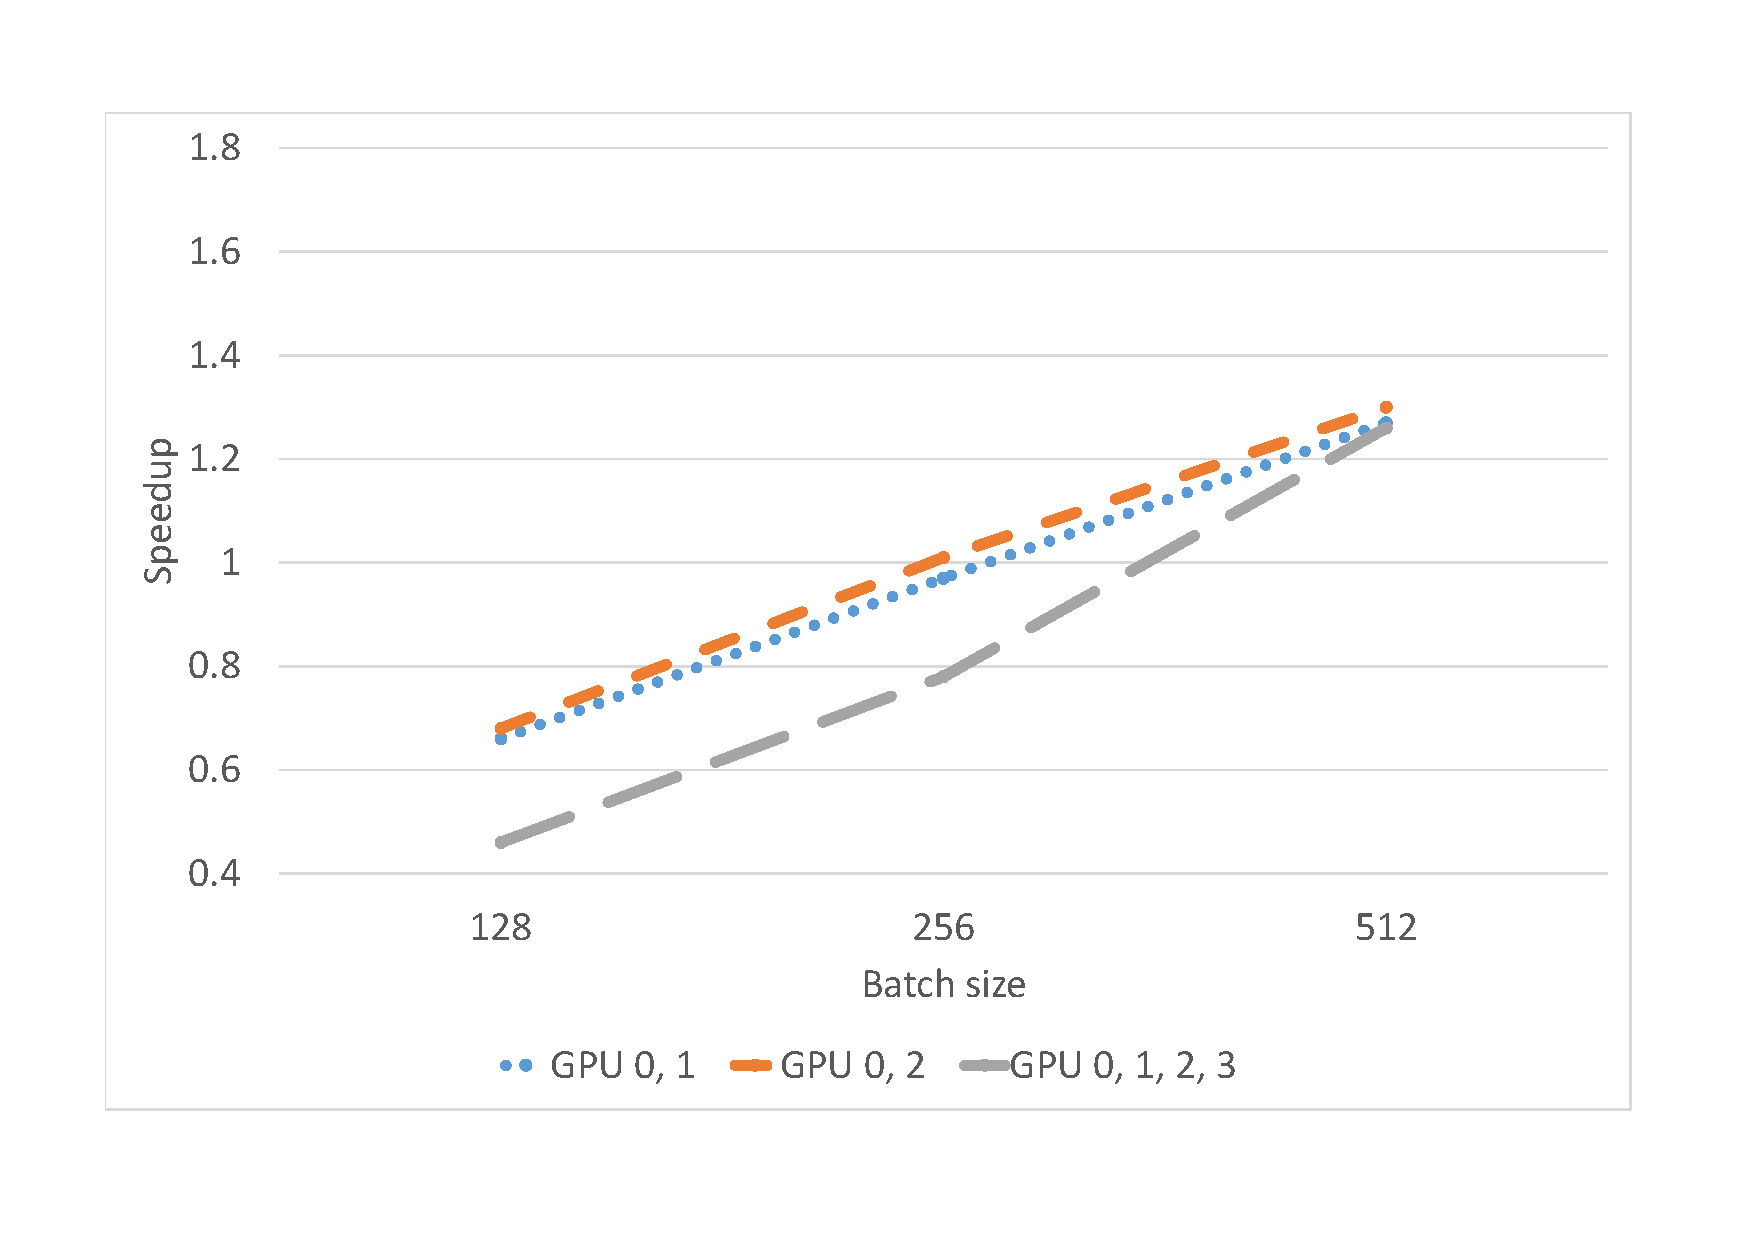
\includegraphics[width=.45\linewidth]{./figures/mg_torch}}
  \subfloat[Caffe execution time]{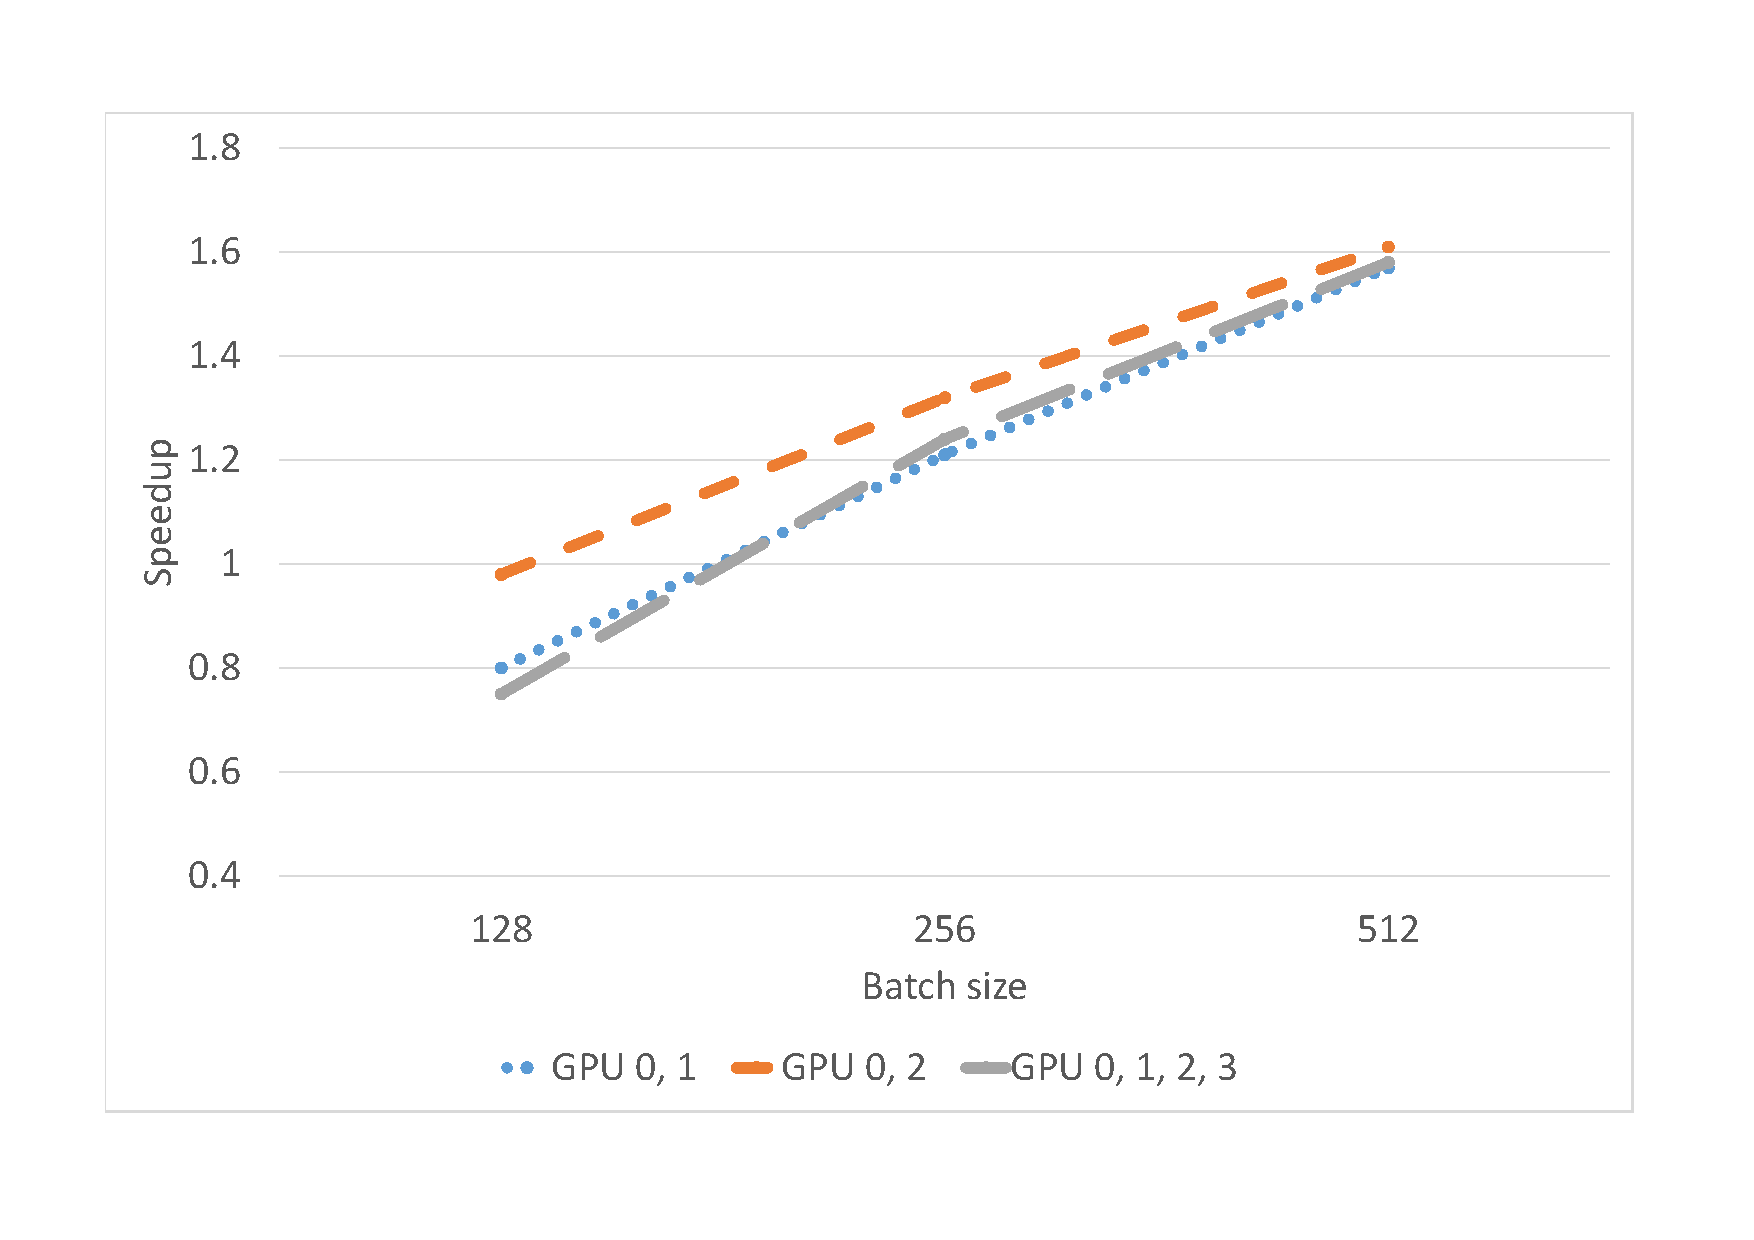
\includegraphics[width=.45\linewidth]{./figures/mg_caffe}}
  \hfil
  \subfloat[TensorFlow execution time]{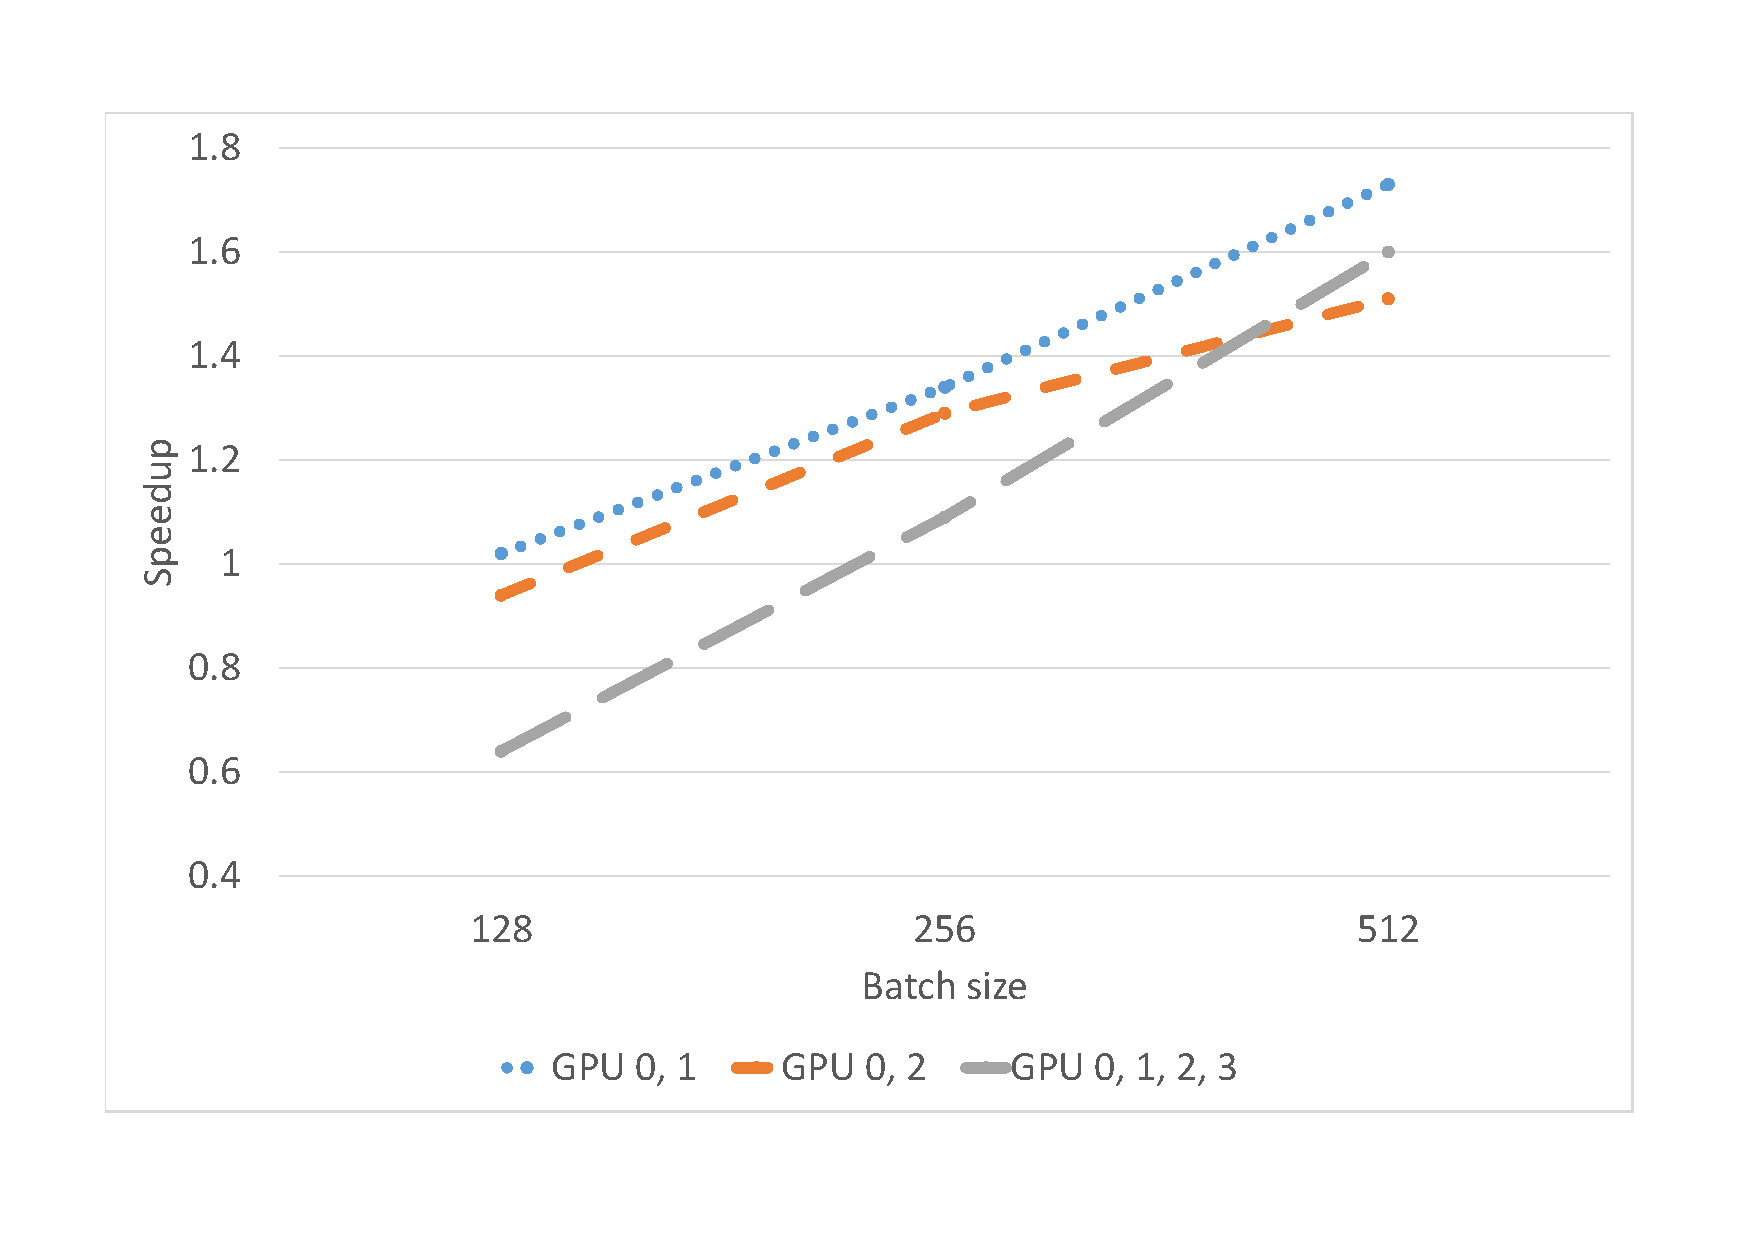
\includegraphics[width=.45\linewidth]{./figures/mg_tf}}
  \caption{%
Speedup of multi-GPU training on each framework.
Here, speedup is calculated by single-GPU execution time of corresponding batch size, divided by multi-GPU execution time.
}
  \label{fig_mg}
\end{figure*}

